\section{Teori}
Jorda er omsluttet av et magnetfelt, som kan tilnærmes med en 
dipolorientert omtrent i flukt med rotasjonsaksen. Jordas magnetiske sørpol 
befinner seg i nærheten av jordas geografiske nordpol, og magnetisk nordpol 
befinner seg i nærheten av geografisk sørpol. Presiseringen "i nærheten av" 
er således viktig i forbindelse med dette prosjektet, ettersom dette gir 
opphav til fenomentet deklinasjon. Et kompass vil peke mot den magnetiske sørpolen og ikke mot den geografiske nordpolen.
Denne misvisningen kalles deklinasjon og blir oppgitt som vinkelen mellom 
geografisk nord og retningen på magnetfeltet. På grunn av asymmetrien til 
de magnetiske polene i forhold til rotasjonsaksen, vil deklinasjonen 
variere og være avhengig av posisjonen på jorda. \cite{World_magnetic_model}

Et annet fenomen er inklinasjon som beskriver hvor mye magnetfeltet peker 
nedover i forhold til horisontalplanet. Ettersom magnetfeltlinjene ikke følger jordas overflate vil 
magnetfeltet peke nedover mot bakken. Inklinasjonen 
blir derfor oppgitt som den vertikale vinkelen mellom tangentplanet til jorda og
magnetfeltet.

\subsection{Phyphox}
Phyphox er en app man kan laste ned på telefonen sin, som lar brukeren 
bruke telefonen sine sensorer til å foreta ulike målinger. Deriblant finnes 
det et magnetometer som lar en måle magnetfelt-styrken langs alle 
koordinataksene til telefonen, i tillegg til absolutt feltstyrke. 
Se https://phyphox.org/ \cite{phyphox} for mer informasjon om sensorer og koordinatsystemet til telefonen.

\subsection{Hvordan måle inklinasjonen}
For å måle inklinasjonen, trenger en kun å finne magnetfelt-styrken i horisontal-
planet og i vertikal retning. Da blir formelen for inklinasjonen 
\begin{equation}
    \gamma = \arctan \frac{-B_z}{B_H} 
\end{equation}
hvor $B_z$ er feltstyrken i z-retning, og $B_H$ er feltstyrken i horisontalplanet, som kan 
uttrykkes med $B_H = \sqrt{B_x^2 + B_y^2}$. $B_x$ og $B_y$ er henholdsvis magnetfeltet i x-retning
og y-retning.
Minustegnet foran $B_z$ kommer av at $B_z$ vil være en negativ størrelse, ettersom magnetfeltet peker inn mot 
jorden, mens 
positiv z-akse står normalt opp fra horisontalplanet. Inklinasjon derimot blir oppgitt 
som en positiv størrelse.
Inklinasjonen blir dermed gitt ved
\begin{equation}
    \label{eq:inclination}
    \gamma = \arctan{ \frac{-B_z}{\sqrt{B_x^2 + B_y^2}} }
\end{equation}

\subsection{Hvordan måle deklinasjonen}
For å finne ut deklinasjonen kreves det at man vet hvor både magnetisk sørpol og 
geografisk nordpol er, for så å kunne regne ut vinkelen mellom dem. For å oppnå dette 
kan det benyttes et mellomsteg, hvor en velger et fast referansepunkt som er enkelt å lokalisere. Dette punktet kan 
en så relatere både magnetfeltet og geografisk nord til. 
Hvis man finner vinkelen mellom magnetfeltet 
og referansepunktet, og geografisk nord og referansepunktet, kan deklinasjonen 
regnes ut basert på dette. Gitt vinklene ovenfor blir deklinasjonen
\begin{equation}
    \alpha = \beta - \theta
\end{equation}
hvor $\beta$ er vinkelen mellom referansepunktet og magnetfeltet, og $\theta$ er 
vinkelen mellom referansepunktet og geografisk nord.

\subsubsection{Vinkel mellom referansepunkt og magnetfelt}
Vinkelen mellom referansepunktet og magnetfeltet kan bli funnet ved å først bestemme et koordinatsystem. I dette 
koordinatsystemet finner en magnetfeltsvektoren og posisjonsvektoren til referansepunktet, og dermed også vinklene 
til vektorene i forhold til x-aksen til koordinatsystemet. Gitt dette oppsettet blir vinkelen mellom x-aksen og 
magnetfeltet 
\begin{equation}
    \phi = \arctan \frac{B_y}{B_x}
\end{equation}
Vinkelen mellom magnetfeltet og referansepunktet blir dermed
\begin{equation}
    \beta = \psi - \phi = \psi - \arctan \frac{B_y}{B_x}
\end{equation}
hvor $\psi$ er vinkelen mellom referansepunktet og x-aksen.

Formelen for deklinasjonen kan dermed skrives om til
\begin{equation}
    \label{eq:Deklinasjon}
    \alpha = \psi - \arctan \frac{B_y}{B_x} - \theta
\end{equation}

\subsubsection{Koordinater til referansepunkt og målelokasjon}
Metoden som brukes for å regne ut vinkelen mellom referansepunktet og geografisk nord, $\theta$ i ligning 
\eqref{eq:Deklinasjon}, krever at man kjenner koordinatene til disse. Dette burde helst bli gjort ved hjelp av 
GPS. Metode-delen av rapporten beskriver hvordan dette ble gjort ved hjelp av telefonens GPS-sensor for 
målelokasjonen samt Google Maps for referansepunktene.

\subsubsection{Vinkel mellom referansepunkt og geografisk nord}

For å finne vinkler på jordoverflaten brukes en ellipsoidisk modell av jorden.
WGS-84 (World Geodetic System) sin referanseellipsoide blir brukt i denne rapporten.
Vinkelen mellom meridianen (linje fra geografisk nordpol til geografisk sørpol) gjennom målelokasjonen og 
kurven fra målelokasjonen til referansepunktet kalles asimut \cite{asimut} og gis ofte symbolet $\alpha$ (se figur \ref{fig:inverse_problem}).
Problemet man står ovenfor da er:
\\

Finn asimuten $\alpha_1$ gitt to punkter på jordoverflaten $(\varphi_1, \lambda_1, )$ og $(\varphi_2, \lambda_2)$, hvor $\varphi$ er breddegradene og $\lambda$ er lengdegradene. 
\\

Dette problemet blir kalt \textbf{Inverse Problem} i \textit{Algorithms for geodesics} (2013) \cite{Karney}. Karney presenterer en metode for å løse slike problemer. Python-biblioteket geographiclib implementerer denne; funksjonen \kode{geodesic.Geodesic.WGS84.Inverse()} tar inn to punkter og løser for geodetisk avstand samt de to asimutene \cite{geographiclib} (se figur \ref{fig:inverse_problem}).

\begin{figure}
    \centering
    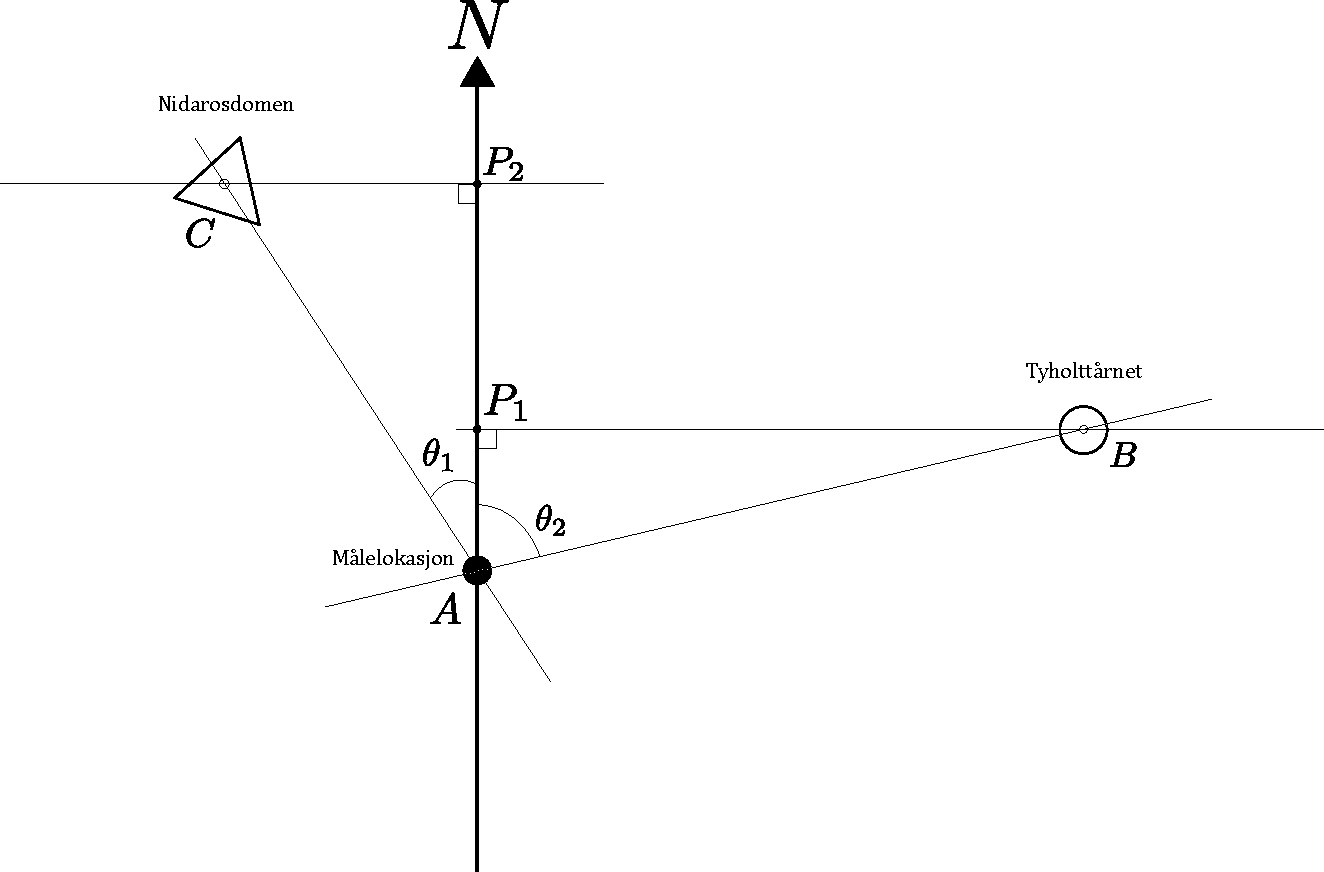
\includegraphics[width=0.75\textwidth]{img/angle_north.pdf}
    \caption{
    Skisse av målelokasjon ($A$) og to referansepunkter ($B$ og $C$) samt vinkelene mellom disse og geografisk nord.}
    \label{fig:angle_north}
\end{figure}

\begin{figure}
    \centering
    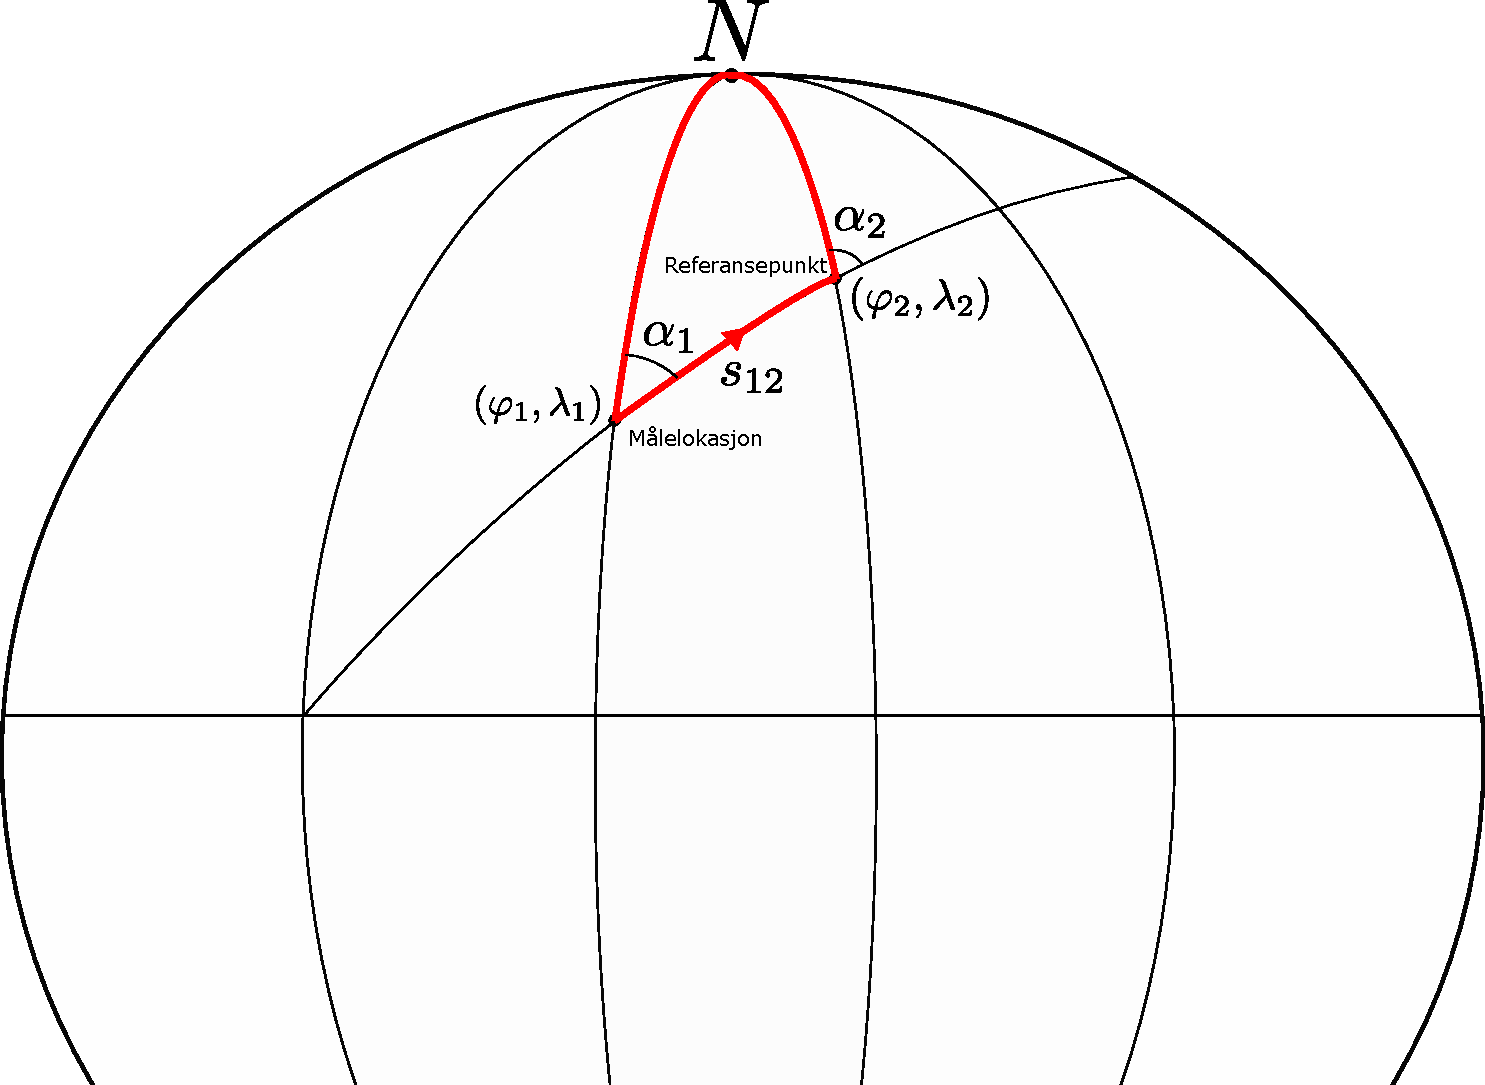
\includegraphics[width=0.75\textwidth]{img/ellipsoidal_problem.pdf}
        \caption{Skisse av en ellipsoidisk modell av jordkloden. Avstanden $s_{12}$ er den geodetiske avstanden mellom to punkter på overflaten. Hvert punkt har en tilhørende asimut ($\alpha$): vinkelen mellom meridianen og den geodetiske kurven.}
    \label{fig:inverse_problem}
\end{figure}
